% ---------
% --------
%!TEX TS-program = pdflatex
%!TEX encoding = UTF-8 Unicode
%!TEX spellcheck = English (Aspell)

\documentclass[11pt]{article}
\usepackage{lucy,handout,graphicx}
\usepackage{fourier-orns}
\usepackage{mathtools}
\usepackage[normalem]{ulem} % either use this (simple) or
\usepackage{tikz}

\def\Cdot{\mathbin{\text{\normalfont \textbullet}}}
\def\Sym#1{\texttt{\color{BrickRed}#1}}
\def\BlueSym#1{\textbf{\texttt{\color{RoyalBlue}#1}}}
\allowdisplaybreaks

\begin{document}

\begin{center}
\Large\textbf{CSCI 332, Fall 2026}%
\\
\LARGE\textbf{Homework 4}%
\\[0.5ex]
\large Due Monday, September 21 Anywhere on Earth (6am Tuesday)
\end{center}

\bigskip
\hrule
\bigskip

\subsection*{Submission Requirements}
\begin{itemize}
    \item Type or clearly hand-write your solutions into a PDF format so that they are legible and professional. Submit your PDF on Gradescope. 
    \item Do not submit your first draft. Type or clearly re-write your solutions for your final submission. If your submission is not legible, we will ask you to resubmit.
    \item Use Gradescope to assign problems to the correct page(s) in your solution. If you do not do this correctly, we will ask you to resubmit.
\end{itemize}

\subsection*{Academic Integrity}

Remember, you may access \EMPH{any} resource in preparing your solution to the homework. However, you \EMPH{must}
\begin{itemize}
    \item write your solutions in your own words, and
    \item credit every resource you use (for example: ``Bob Smith helped me on
    this problem. He took this course at UM in Fall 2020''; ``I found a solution
    to a problem similar to this one in the lecture notes for a different
    course, found at this link: www.profzeno.com/agreatclass/lecture10''; ``Here is a link to the full transcript of my chat with ChatGPT about the problems on this HW''.)
    Ask if you need any clarifications about how to properly cite your sources!
\end{itemize}




\newpage
%----------------------------------------------------------------------

\headers{CSCI 332}{Homework 4 (due September 21)}{Fall 2026}


\begin{enumerate}
%\parindent 1.5em \itemsep 4ex plus 0.5fil

%----------------------------------------------------------------------

\item (0 points) List the resources you used for each problem in this homework. If you used no resources except
lecture notes and videos and the linked textbook, you can say ``none''. If you used
an AI tool, you should put a link to your full conversation here, and you must
use the
\href{https://umaal.org/files/teaching/csci332_fall2026/agents.md}{provided
prompt}
 to guide the AI to act
as a tutor, not an answer-provider.

You will be asked to resubmit your homework if this section is blank.

Remember that no matter what resources you consulted, you must write your solutions
\emph{in your own words}.

\item (1 point) (without (b), 2 points) Write the reucrrence describing the following algorithm's runtime.
(That is, fill in the blanks below.)

\begin{algo}
    Alg(array $A$ of length $n$):\+ \\
        If $n = 1$: \+ \\
            Return $A$ \- \\
        Else: \+ \\
            Return Alg(array formed by taking the values at odd indices of $A$)
\end{algo}

    \begin{equation*}
        T(n) =
        \begin{cases}
        \underline{\hspace{3in}} & if n \underline{\hspace{1in}} \\
        \underline{\hspace{3in}} & if n \underline{\hspace{1in}} \\
        \end{cases}
    \end{equation*}
\item \sout{(3 points) Using induction, prove that the sum of the degrees of all vertices in an
undirected graph is equal to two times the number of edges in the graph.
To earn any points, your proof must use the exact form we learned in class on
Friday (universal declaration, inductive hypothesis, cases, wrap-up statement.)}
\item (6 points) (without (b), 8 points) Suppose you are given a stack of $n$ pancakes of different sizes. You want to
sort the pancakes so that smaller pancakes are on top of larger pancakes.
The only operation you can perform is a \emph{flip}---insert a spatula
under thet top $k$ pancakes, for some integer $k$ between 1 and $n$, and flip them all over.

\begin{figure}[h!]
    \begin{center}
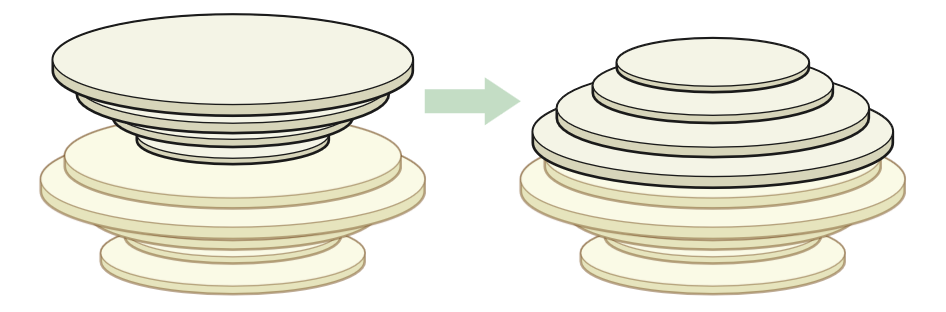
\includegraphics[width=.5\textwidth]{pancakes.png}
    \end{center}
    \caption{Flipping the top four pancakes.}
\end{figure}

\begin{enumerate}
    \item Let $PancakeSort$ be an algorithm that sorts a stack of pancakes. Given a stack of
    $n$ pancakes $S$, describe how you could perform a constant number of flips on $S$
    so that calling $PancakeSort$ on the top $n-1$ pancakes completes the sorting of $S$.
    \item Write the full recursive $PancakeSort$ algorithm.
    \item Write the recurrence for your $PancakeSort$ algorithm's runtime $T(n)$.
\end{enumerate}



\end{enumerate}
%%%%%%%%%%%%%%%%%%%%
\end{document}
